% !TEX TS-program = pdflatex
% !TEX encoding = UTF-8 Unicode

% This is a simple template for a LaTeX document using the "article" class.
% See "book", "report", "letter" for other types of document.

\documentclass[11pt]{article} % use larger type; default would be 10pt

\usepackage[utf8]{inputenc} % set input encoding (not needed with XeLaTeX)

%%% Examples of Article customizations
% These packages are optional, depending whether you want the features they provide.
% See the LaTeX Companion or other references for full information.

%%% PAGE DIMENSIONS
\usepackage{geometry} % to change the page dimensions
\geometry{a4paper} % or letterpaper (US) or a5paper or....
\geometry{margin=1in} % for example, change the margins to 2 inches all round
% \geometry{landscape} % set up the page for landscape
%   read geometry.pdf for detailed page layout information

\usepackage{graphicx} % support the \includegraphics command and options

\usepackage[parfill]{parskip} % Activate to begin paragraphs with an empty line rather than an indent
\setlength{\parindent}{1cm}

%%% PACKAGES
\usepackage{booktabs} % for much better looking tables
\usepackage{array} % for better arrays (eg matrices) in maths
\usepackage{paralist} % very flexible & customisable itemizes (eg. enumerate/itemize, etc.)
\usepackage{verbatim} % adds environment for commenting out blocks of text & for better verbatim
\usepackage{subfig} % make it possible to include more than one captioned figure/table in a single float
\usepackage{amssymb} % more 'unusual' symbols not included in standard LaTeX package
\usepackage{enumitem}
\usepackage{amsmath}
\usepackage{comment}
\usepackage{color}
\usepackage{graphicx}
\usepackage{xspace}
\usepackage{gensymb}
\usepackage[font=small,format=plain,labelfont=bf,textfont=normal,justification=justified,singlelinecheck=false]{caption}
\usepackage{calligra}
\DeclareMathAlphabet{\mathcalligra}{T1}{calligra}{m}{n} 
\DeclareFontShape{T1}{calligra}{m}{n}{<->s*[2.2]callig15}{} 

% These packages are all incorporated in the memoir class to one degree or another...

%%% HEADERS & FOOTERS
\usepackage{fancyhdr} % This should be set AFTER setting up the page geometry
\pagestyle{fancy} % options: empty , plain , fancy
\renewcommand{\headrulewidth}{0pt} % customise the layout...
\lhead{}\chead{}\rhead{}
\lfoot{}\cfoot{\thepage}\rfoot{}


%%% SECTION TITLE APPEARANCE
\usepackage{sectsty}
\allsectionsfont{\sffamily\mdseries\upshape} % (See the fntguide.pdf for font help)
% (This matches ConTeXt defaults)

%%% ToC (table of contents) APPEARANCE
\usepackage[nottoc,notlof,notlot]{tocbibind} % Put the bibliography in the ToC
\usepackage[titles,subfigure]{tocloft} % Alter the style of the Table of Contents
\renewcommand{\cftsecfont}{\rmfamily\mdseries\upshape}
\renewcommand{\cftsecpagefont}{\rmfamily\mdseries\upshape} % No bold!

%%%Command Macros


%%% END Article customizations

\graphicspath{ {./images/} }

\title{The Mimas Leading Edge Anomaly: Thermal conductivity and grain cementation radius estimation}
\author{M.J. Schaible, R.Johnson, L. Zhigilei}
%\date{} % Activate to display a given date or no date (if empty),
         % otherwise the current date is printed 

\begin{document}
\maketitle

\section{Abstract}

	Goals:
	\begin{itemize}
	\item Explain the thermal conductivity differences between inside/outside anomalous region on Mimas and Tethys
		\begin{itemize}
		\item Can the thermal conductivity differences be explained in terms of structural differences in the regolith?
		\item How does the thermal conductivity depend on grain contact, linear or quadratic?
		\item Is Hertzian analysis sufficient to determine effective contact areas between grains?
		\end{itemize}
	\item Estimate effects of $>$1MeV electrons on grain cementation properties
		\begin{itemize}
		\item What is the deposition profile of the electrons in the regolith?
		\item How does electron/target interaction energy change with depth?
		\item What is the heating effect on $\sim$50$\mu$m grains for each interaction?
		\item Are molecules desorbed from the pore surfaces? Can we determine an average per interaction?
		\item Is internal diffusion enhanced?
		\item Is the crystal structure at the grain boundary affected? How is thermal conductivity changed?
		\item Does the average number of molecules desorbed/diffused vary with depth in the regolith or proximity to pore surface?
		\end{itemize}
	\item Estimate time-scale for cementation increase to explain increased cementation
	\item Estimate gardening rate due to micrometeorite bombardment to counteract the sintering process
	\end{itemize}

	Thermal conductivity models have been developed to model heat transport in planetary and cometary surfaces. These models depend on the thermal conductivity of the bulk material making up the regolith ($k_{bulk}$) the porosity ($\phi$) and on geometric factors that depend on the packing of grains. For the case of an icy regolith on an airless body in the outer solar system, contributions to thermal conductivity other than conduction through grains (i.e. radiative, convective, latent heat) can be shown to be negligible.

\newpage
\section{Introduction}
\label{sec:intro}

	Analysis of Cassini photometry data revealed an anomalous region present on the leading edge of the Saturnian icy moons Mimas and Tethys. That such a feature would exist was first suggested during the Voyager-era when a dark equatorial band across the leading hemisphere of Tethys was identified. A lens shaped feature symmetric with respect to the center of the leading hemisphere and the equator on both Mimas and Tethys (and possibly Enceladus) was seen clearly by the ISS (Imaging Science Subsystem) on Cassini as a low IR/UV ratio compared to the remainder of the leading hemisphere [Shenketal2011]. The feature extends the entire width of the leading hemisphere and $\sim \pm40\degree$ and $\sim \pm20\degree$ to the north and south at the center of the lens for Mimas and Tethys respectively, though it narrows to within a few degrees at the edges of the hemisphere for both moons. The feature was dark in the IR (0.930 $\mu$m) and Green (0.568 $mu$m) light bands but bright in the UV (0.338 $\mu$m) as shown by albedo maps [Elderetal2007; Shenketal2011]. The smaller IR/UV ratio in the anomalous region was explained as increased scattering at UV wavelengths due to a higher concentration of light scattering defects in the icy regolith grains, possibly caused by preferential energetic particle bombardment in that region.
	
	The CIRS (Cassini InfraRed Spectrometer) instrument which measured the mid-IR regime subsequently showed that surface temperature variations during the day and night cycle, determined by measurements of thermal emission, within a lens shaped region consistent with that identified in by the color maps, were greater than the surrounding area, indicating a greater thermal conductivity of the material in the lens shaped region [Howettetal2011]. The location of the anomaly was shown to closely match the expected deposition profile of high energy ($\>\approx$1 MeV) electrons rapidly moving along the magnetic field lines perpendicular to the rotational plane of the moons [Paranicasetal2012]. The electrons move with a high bounce frequency such that they are condensed out as soon as the magnetic field line crosses the surface and, unlike the thermal plasma, travel with their net guiding center of motion opposite the rotation direction of the Mimas and Tethys and thereby deposit energy preferentially on the leading edge of these bodies. It was hypothesized that the electrons could create scattering centers in the icy regolith, leading to the observed IR/UV discolorations. Furthermore, the surfaces of the moons are composed almost entirely of crystalline water ice, while essentially free of organic species [Filacchioneetal2010], and the energy deposition due to these electrons could cause sintering of the icy regolith grains leading to increased heat transfer and thus explaining the anomalous thermal inertia.

	A good deal of thermal modeling has been done to understand the structure of comets and the thermal inertia of other bodies such as the Moon and Mars. However, the Saturnian moons are composed of water ice as opposed to a rocky regolith and lack the dark organic layer which found on the surface of comets. Also, since the moons lack an atmosphere the thermal conductivity is dominated by intergrain contacts while the thermal conductivity due to gas convection in the regolith is negligible. The purpose of this note is to quantitatively estimate the expected relative contact area or grain sintering radius based on the measured parameters of thermal inertia and grain size. The estimate assumes that both the ice grains and the cementation volume is entirely crystalline. Although amorphous ice could be present, the effect on thermal conductivity of the crystalline to amorphous transition is shown to be a much smaller effect than the increase in surface area. The structure of the ice will be discussed in more detail later in this note. 
	
	%REJ - One nice thing would be to correlate defect production--determining the IR/UV ratio to energy deposition--for which there are expressions and then show that that amount of energy deposition is also consistent with your model of the sintering 

\subsection{Thermal Inertia ($I$) and Skin Depth ($\delta$)}

		Using measured surface thermal emission excursions values for thermal inertia $I=\sqrt(kc\rho)$ were extracted by Howett et al. (2011, 2012). Using these values and assuming a porosity of $\phi = 50\%$, the thermal conductivity and the skin depths $\delta = \frac{I_{out}}{(1-\phi)\rho_{ice} c \sqrt{\omega}}$ inside and outside the anomalies were determined and are given in Table 1, where $c$ is specific heat taken as 0.82 MKS, $\rho_{ice}$ is the density of bulk ice (0.934 g/cm$^{3}$), and $\omega$ the angular velocity of rotation. The skin depth of calculated assumes that the conductivity is that of porous, crystalline ice regolith. However, the contact area between grains formed by sintering could have different conductivity. 
	
	\begin{table}[h]
		\centering
		\begin{tabular}[c]{ l | l | c | c | c }
		Body & Location & Thermal Inertia & Skin Depth & Thermal Conductivity \\
		& & $\left[ \frac{J}{m^{2} s^{1/2} K} \right]$ & [cm] & $\left[ \frac{J}{m\cdot s\cdot K} \right]$ \\ \hline
		Mimas & Inside anomaly & 66 $\pm$23 & 2.01 $\pm$0.7 & 1.13 $\left(\substack{+0.94 \\ -0.65} \right) \times$ 10$^{-2}$ \\
			& Outside anomaly & $<$16 & $<$ 0.49 & $<$ 6.7 $\times$ 10$^{-4}$) \\ \hline
		Tethys & Inside anomaly & 25 $\pm$3 & 0.76 $\pm$0.09 & 1.63 $(\pm 0.4) \times$ 10$^{-3}$ \\
			& Anomaly boundary & 11 $\pm$1 & 0.34 $\pm$0.03 & 3.16 $(\pm 0.6) \times$ 10$^{-4}$ \\
			& Outside anomaly & 5 $\pm$1 & 0.15 $\pm$0.03 & 6.53 $\left(\substack{+2.9 \\ -2.4} \right) \times$ 10$^{-5}$ \\
		\end{tabular}
		\caption{Calculated thermodynamic values for the surface materials of Mimas and Tethys. Values of thermal inertia were taken from Howett et al. (2011, 2012) and basic equations were used to calculate the remaining quantities.}
		\label{tab:therm}
	\end{table}
	
	The average path length traveled by $1 - 10 MeV$ electrons impacting on water, calculated with the ESTAR program using the continuous-slowing-down-approximation (CSDA), is $0.4-5.0 g/cm^{2}$, which for $50\%$ porous water ice gives $0.85-10.6 cm$ total path length [NIST, e-star]. The depth of penetration into the material must be less than the total path length, but due to efficient scattering effects from electron-nucleus and electron-electron interactions, the actual electron penetration depth varies. For light materials such as water ice, the maximum depth is expected to be on the order of the CSDA range [Attix, 2008]. \emph{The program PENELOPE was developed to simulate the implantation of electrons into materials and was used to generate a plot of the electronic stopping power and range of electrons into water (\~ref{fig:ewater}). I don't actually plan to leave these images in. They are just placeholders while I am working on simulations using the PENELOPE program to simulate MeV electron irradiation of water. I will update when I have more progress.}
	
	\begin{figure}[h]
	\centering
		\subfloat{{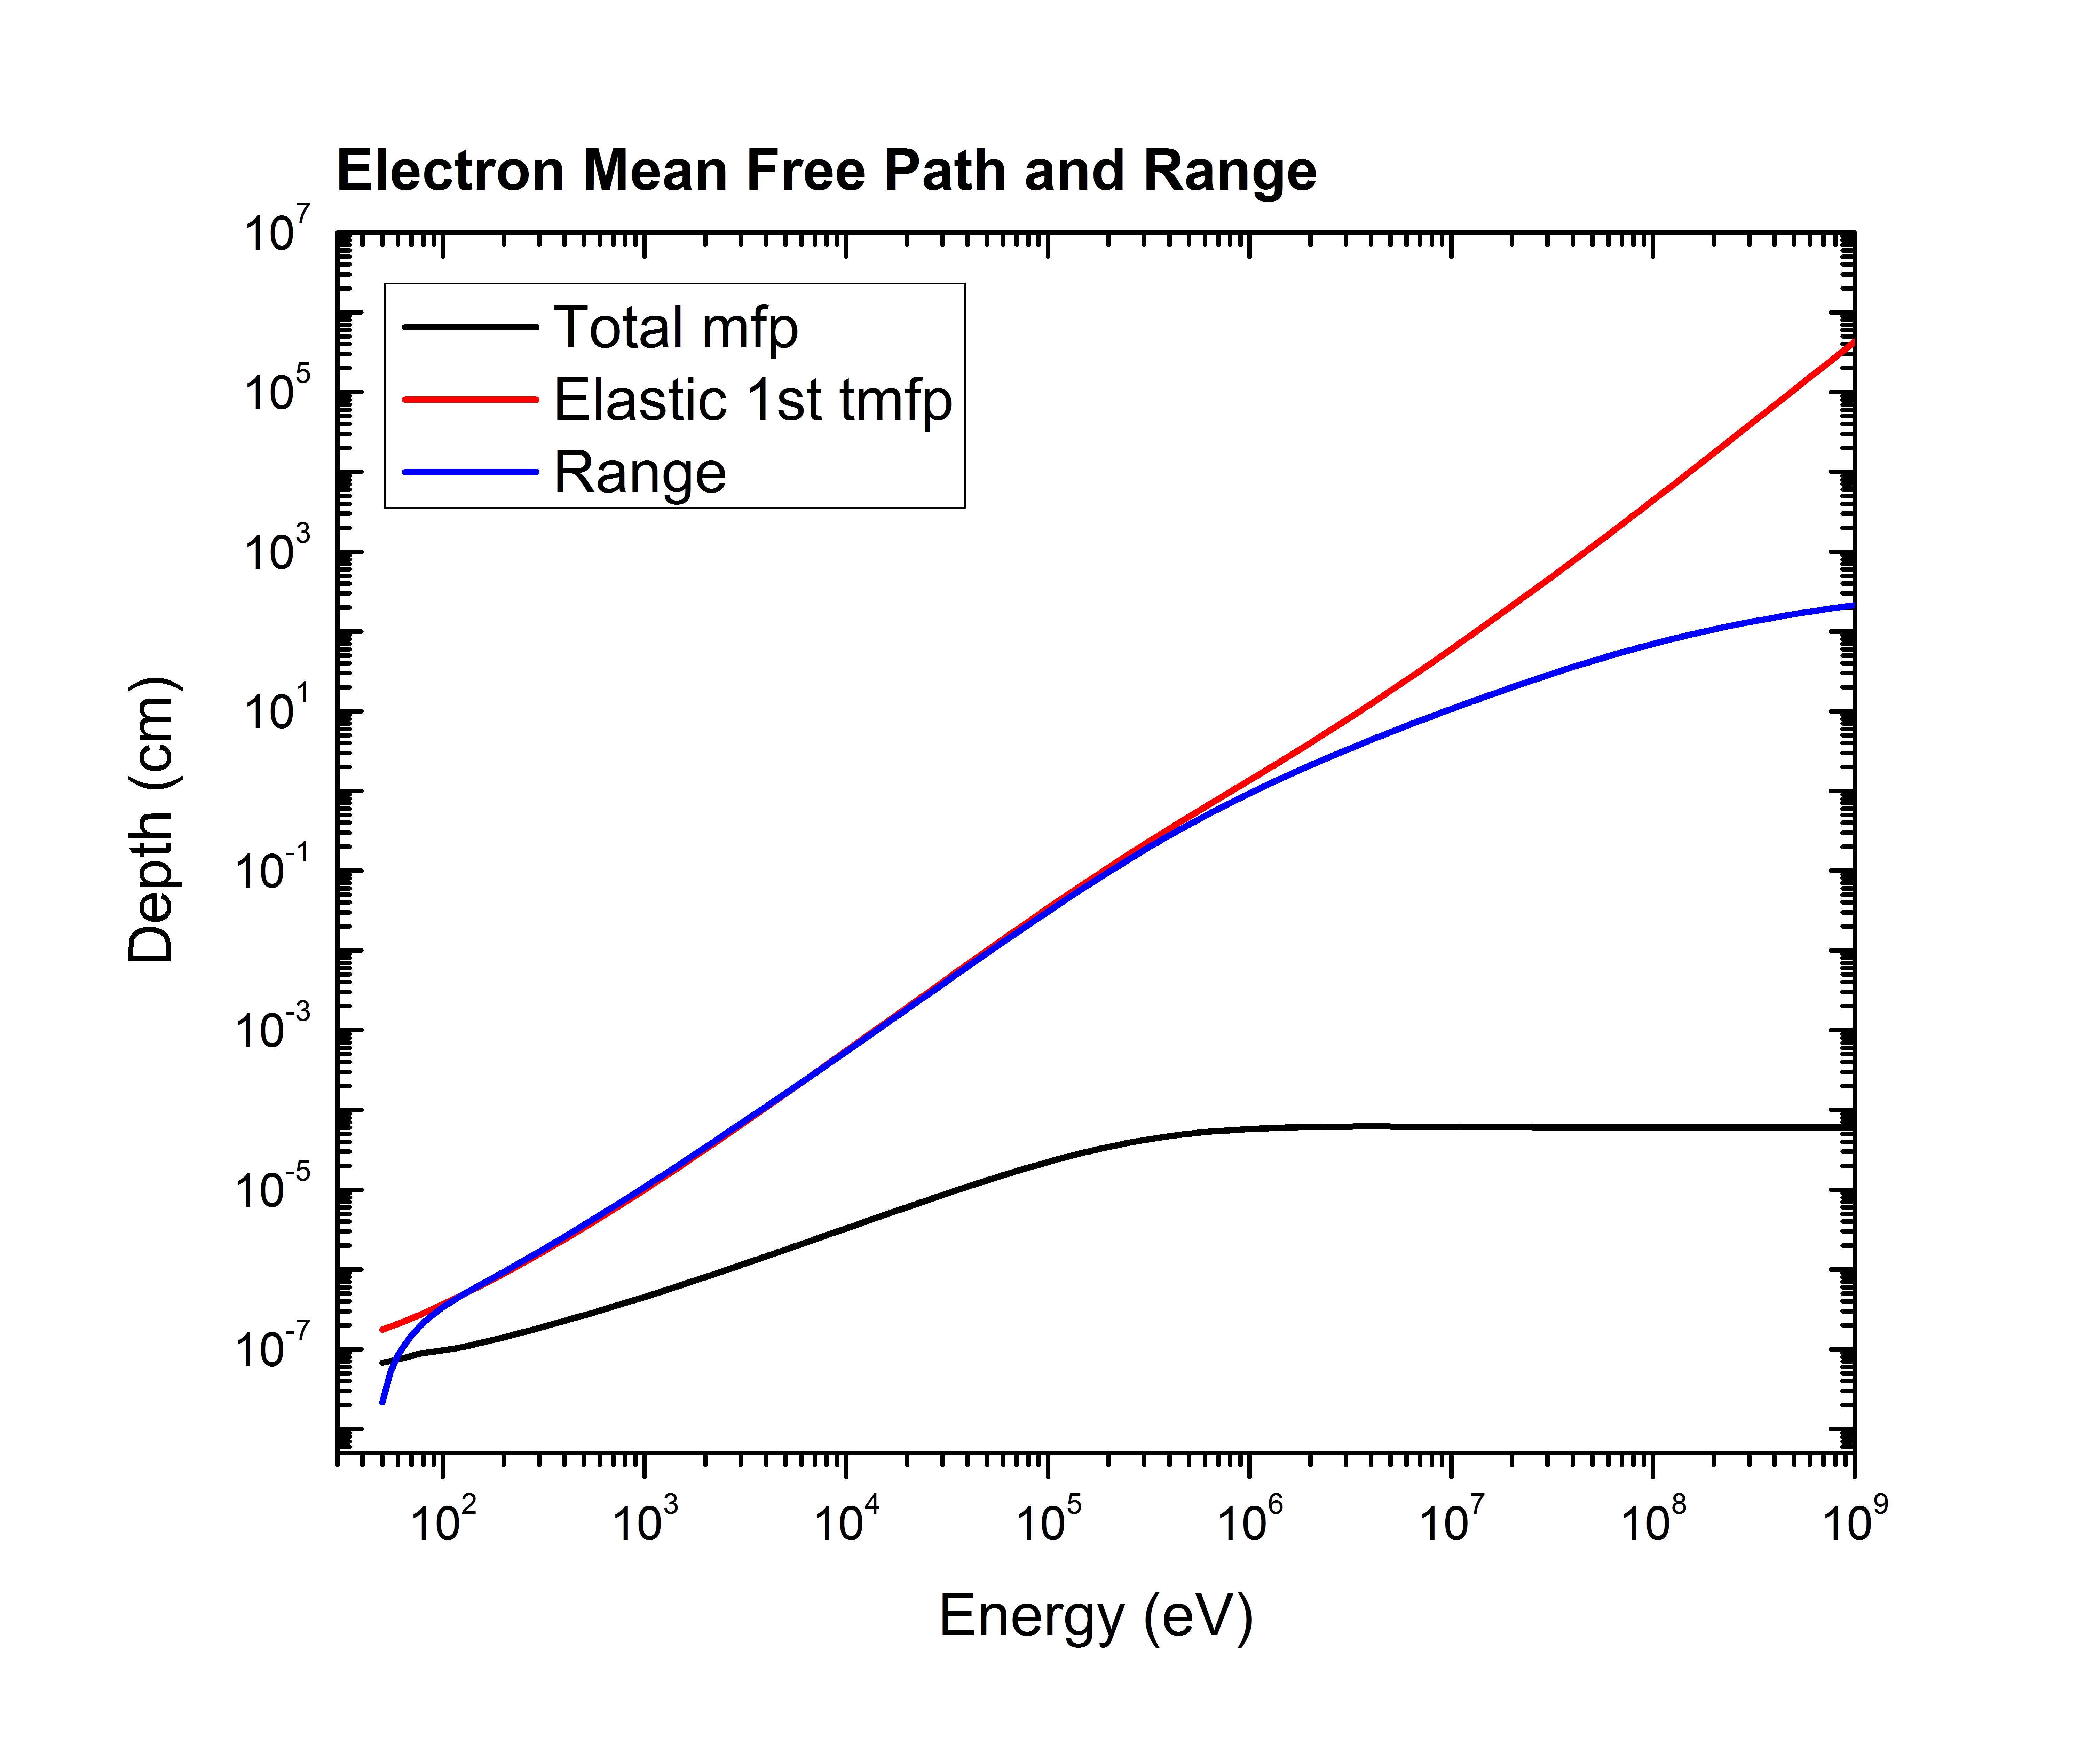
\includegraphics[width=0.45\textwidth]{elec_range.png} }}
		\subfloat{{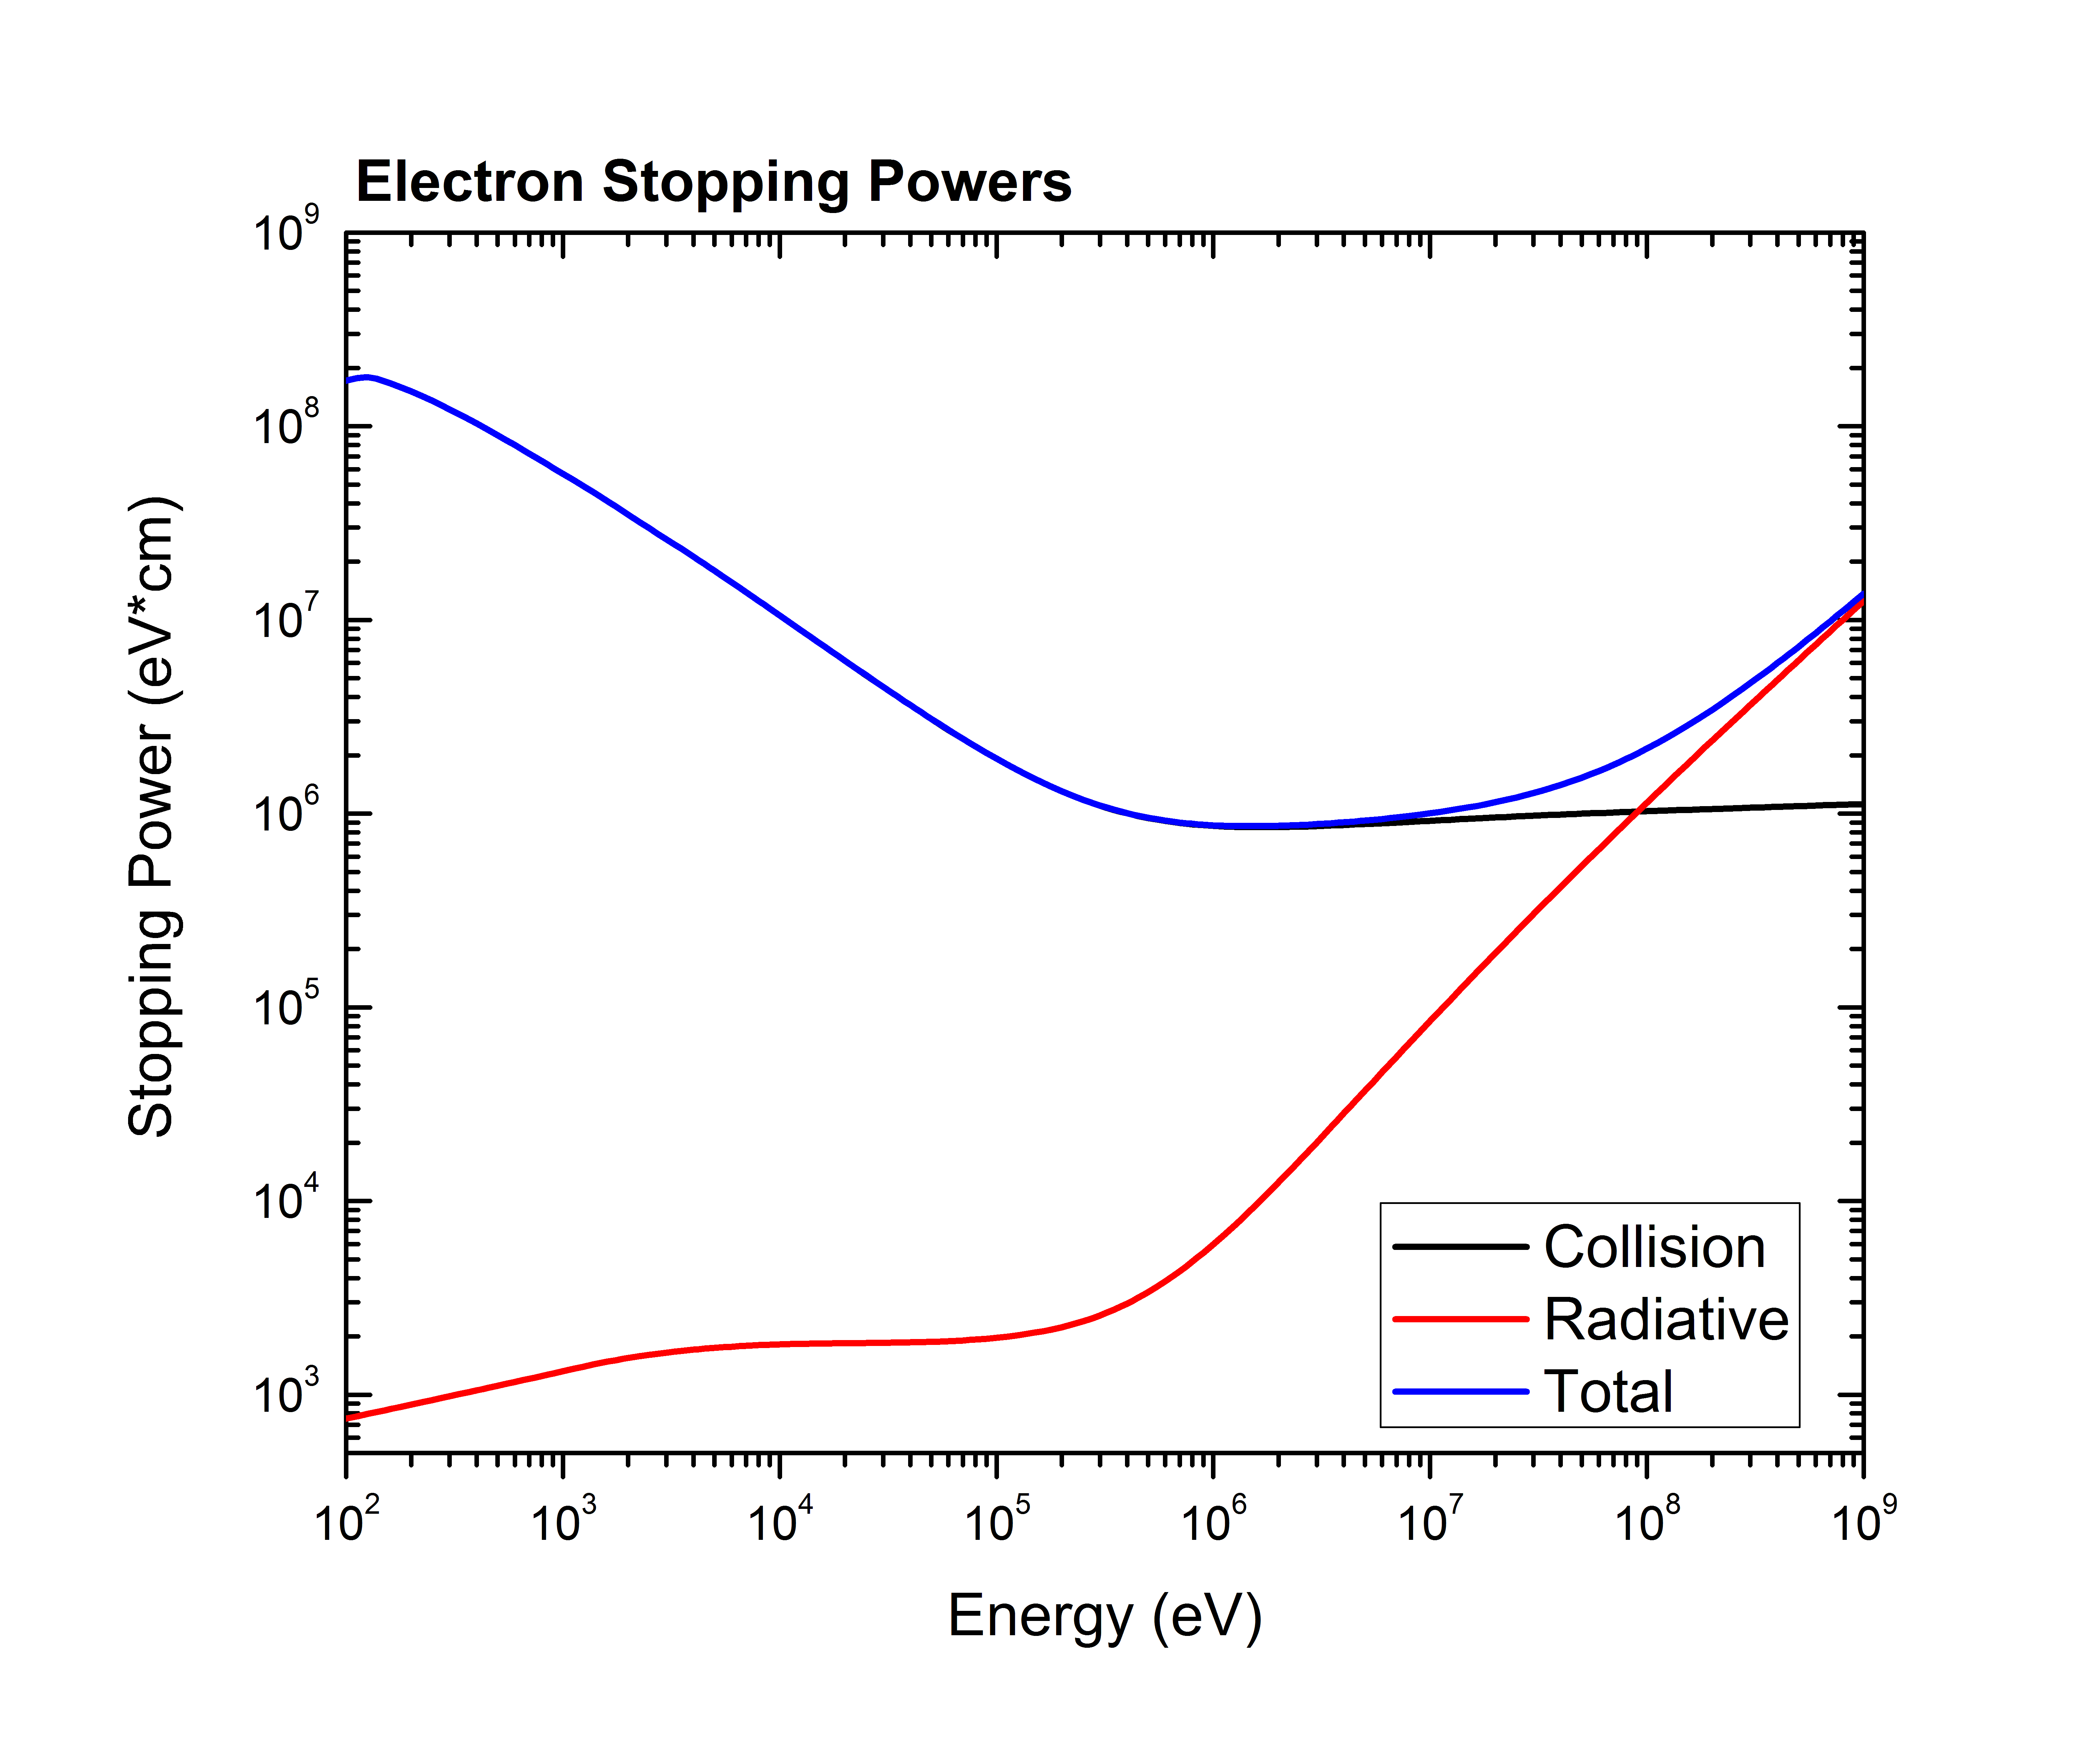
\includegraphics[width=0.45\textwidth]{elec_stp.png} }}
	\caption{Electron range and stopping power calculated for pure water.}
	\label{fig:ewater}
	\end{figure}
	
	The similarity in the penetration depths of the electrons and the skin depth of the thermal anomaly suggest that the electrons could be responsible for the increased thermal conductivity.  Here we consider that a possible explanation for the thermal conductivity differences could be sintering between adjacent regolith grains driven by energy deposited in electronic excitations of the water molecules either on the surface or in the bulk of the ice grains. The deposited energy can mobilize water molecules, causing them to migrate along the grain surface, through the bulk, or desorb from the surface and reabsorb in the intergrain region. This can lead to grain growth and, more importantly, growth in the size of the contact regions between grains and improved thermal contact  across the grain boundaries.
	
	 As discussed below the same energy deposition that mobilizes the water at the grain boundaries can cause defects in the bulk. Whereas sintering increases the effective thermal conductivity, such defects, which we assume to be the principal cause of the increase in the IR/UV ratio[ref], can cause a decrease in thermal conductivity. However, below we will also show that the density of bulk defects produced at a level consistent with the sintering are sufficient enough to affect the UV scattering but not to significantly decrease the thermal conductivity.
	
%\emph{There should be a pressure minimum in the pendular region. Need equation to explain. Another argument in the minimization of surface energy. Need to look more into that too.}
	
\section{Contributions to the effective thermal conductivity of an icy porous regolith}

	In general, the effective thermal conductivity of a granular, uncemented sample under vacuum can be separated into a conductive component which describes heat flow through the bulk and a radiative term which describes heat flow through the void space [Watson, 1964]. 
	
	\begin{equation} \label{eq:TCbasic}
	k_{eff} = k_{rad}(T^{3}) + k_{cond}
	\end{equation} 
	
	The first term depends on both grain size and porosity and is due to radiation as discussed further below. The second factor was given by Watson (1964) as $k_{cond} = \frac{3000}{r_{g}}\times10^{-5}$ for $r_{g} > 20 \mu m$ and is a function of the bulk conductivity of the grain material ($k_{g}$) and the contact area ($S$) between grains. For cold, porous regoliths typical of airless solar system bodies in the outer solar system, heat flow is limited by the amount of intergrain contact.

	In general, $k_{rad}$ and $k_{cond}$ can depend on factors such as grain size, porosity, temperature, packing structure etc. Additionally, molecular desorption and feedback heating can raise the gas pressure in the pore space giving an additional convective path for heat transfer between grains ($k_{conv}$). Thermal conductivity measurements and modeling using either a spherical grain approximation or continuum techniques can be used to parameterize the variables for analytical expressions. However, much work has been done to constrain the various parameters that affect the thermal conductivity, and those possibly relevant to Mimas and Tethys will be outlined and their usefulness for describing the effective thermal conductivities reported by Howett et al., (2011, 2012) is discussed below.
	
%	Computationally, though variations in porosity, vacuum conditions, and grain size can be difficult to study in the lab and using solid sphere computational models may miss important effects from the regolith microstructure.

\subsection{Radiative contribution to thermal conductivity}

	The contribution to the effective thermal conductivity from radiative heat emission from the grain/pore surfaces, $k_{rad}$, can be estimated as [Kasparek and Vortmeyer, 1976]

	\begin{equation}
	k_{rad} = 4 \psi r_{g} \sigma T^{3}
	\end{equation}
	
	where $r_{g}$ is the particle diameter, $T$ is the temperature, $\sigma$ is the Stephan Boltzmann constant, and $\psi$ is a heat transport coefficient defined by
	
	\begin{equation}
	\psi = \frac{2F + \epsilon'(1-F)}{2(1-F)-\epsilon'(1-F)}
	\end{equation}

	for which F is a 'radiative constant' equal to $\approx$ 0.08 and $\epsilon'$ is related to the emissivity $\epsilon$ of the material by $\epsilon' = \frac{\epsilon}{\epsilon +0.5(1-\epsilon)}$. Taking $r_{g} = 50 \mu m$, and $\epsilon = 1$, then the radiative contribution to the thermal conductivity can be estimated as $k_{rad} \approx 6.3\times10^{-6} \frac{J}{m \cdot s \cdot K}$.
	
	Thus we see that the radiative contribution at approximate Mimas temperatures can account for only $\approx 1/3000$th of the total thermal conductivity as measured for the anomalous region on Mimas. Though it could account for as much as 1/10th of the thermal conductivity outside of the anomalous region on Tethys, it is typically on the order $<1\%$ contribution to the total thermal conductivity and will be neglected in the remainder of our analysis.

\subsection{Latent heat contribution to thermal conductivity}
	An additional mechanism not considered by watson (1964) in Eq.\ref{eq:TCbasic} is heat transfer due to molecular desorption and re-absorption within pores, i.e. sublimation, the expectation being that there is a higher rate of sublimation on the high temperature side of the pore and thus heat conductivity across the void space. We can model the sublimation process using the Hertz-Knudsen formula [ref]:

	\begin{equation}
	k_{lat} = ( \frac{\mu}{2 \pi k_{B} T})^{1/2}  (L S) \frac{dP}{dT}
	\end{equation}
	
	where $m$ is the molar mass of the gas molecule, $k_{B}$ is the Boltzmann constant, $L$ is the latent heat of sublimation per unit mass and $S = \phi r_{g}$ is the average pore size dimension where $\phi$ is the porosity and $r_{g}$ the average particle diameter. The vapor pressure $P$ of the gas of interest is given by the Clausius-Clapeyron equation:
	 
	 \begin{equation} \label{eqn:CCpres}
	 P = ae^{(-b/T)}
	 \end{equation}
	 
	 where $a$ and $b$ are experimentally determined parameters for water vapor over ice given by Fanale et al. (1984) as $a = 3.56 \times 10^{13} dyne/cm^{2}$ and $b = 6141.667 K$. Taking the latent heat of sublimation to be $L = 48600 [\frac{J}{mol}]$ and again using a temperature of 80 K, the contribution to thermal conductivity from the latent heat is $k_{lat} = 1.15\times10^{-26} MKS$. Though at low temperatures this effect is negligible, Steiner and K\"{o}mle (1991) showed that it should be included at temperatures above ~170K. At the temperatures considered here the net thermal conductivity of the grains is controlled the second term in Eq.\ref{eq:TCbasic} and is modeled as due to solid state heat transfer.

\subsection{Solid state heat transport models for a porous icy regolith}
	There are several methods in the literature for estimating solid state heat transfer in a grainy regolith that take into account grain size, porosity, and a cementation or contact area between adjacent grains. For cold grainy regoliths, heat flow is limited by the intergrain contact area which in turn depends on the crystalline and defect structures of the cementation region or grain boundaries. In the following we will review several approaches to modeling the thermal conductivity of an icy regolith including cementation between grains. All of the thermal conductivity models considered here incorporate an effective contact radius into equations for the effective thermal conductivity. The contact radius is either obtained directly through Hertzian analysis (discussed below) or through use of a proxy 'Hertz-factor'. Taking the measurements of effective thermal conductivity for the moon surfaces and making reasonable assumptions about packing structure and porosity, grain size, thermal conductivity of the grain materials, the effective contact area between grains for the areas inside and outside the anomalous regions can be compared for the various models. Then it can be determined if the energy deposition from the MeV electrons is sufficient to explain the larger relative contact area within the anomalous region.

\subsubsection{Hertz-factor description of grain contact area}
	In modeling of thermal conductivity of grainy and porous materials, a common approximate technique is to consider a mono- or polydisperse 'bed' of elastic spheres. The requirement for the spheres to be elastic and not a perfect hard sphere stems from physical considerations, since the contact point of hard spheres is infinitesimal, through which no heat can flow, meaning that the spheres must deform slightly at the contact point so there is some finite area across which heat can flow. At the atomic scale, the heat transfer through dissimilar spheres with no rigid bonding is due predominantly to the van der Waals interactions which mediate the phonon transfer, while for cemented grains heat is transfered directly through lattice vibrations. Deformation between curved, elastic surfaces in contact was first studied by Heinrich Hertz in 1882, and Hertzian analysis can be used to determine the intergranular contact area and indentation depth of the surfaces. The radius of the contact between two spheres depends on the material properties and is related to an applied load $F$ by:

	\begin{equation}
	R_{con,eff} = \left[ \frac{3}{4} \frac{1 - \nu^{2}}{E(T)} r_{g} F \right]^{1/3}
	\end{equation}

	where $\nu$ and $E(T)$ are Poisson's ratio and Young's modulus of the material, respectively. The applied load determines how strongly adjacent particles are bonded and, for a loose regolith, the weight of the grains can be used to determine the force and thus the contact area. However, gravitational forces in the near surface region are negligible as compared to van der Waals bonding which provides orders of magnitude greater adhesive interactions. The adhesive force is effectively the tensile load at the point where the spheres are separated and can be calculated by JKR theory [Johnson et al., 1971].
	 
	 \begin{equation}
	 F_{JKR} = 3 \pi \gamma_{s} r_{g}
	 \end{equation} 
	 
	 where $\gamma_{s}$ is the specific surface energy of the material. Hertzian analysis can be used in thermal conductivity expressions for non-cemented grains to describe the effective radius of the intergranular contact and make comparisons for otherwise identical regoliths to determine the relative area through which heat can flow. A larger contact radius corresponds to greater interparticle contact, thereby allowing a greater heat flux and a higher thermal conductivity. It should be noted here that these expressions may not be applicable for cemented grains where the intergrain boundary may have some degree of crystalline bonding. Instead, thermal conductivity in these instances can be modeled by taking into account of cementation area which will continue to be the limiting factor in heat transfer through the regolith grains. 

	By taking the Hertzian contact radius to be the ratio of the effective and bulk thermal conductivities $R_{con} = k_{eff}/k_{ice}$ and assuming other materials parameters as well as the packing structure are the same inside and outside the anomaly, the ratio of the grain size inside and outside the anomaly necessary to determine the measured thermal conductivity differences can be determined. At lower temperatures where radiative heat transfer is negligible, the thermal conductivity $k_{eff} \varpropto (r_{g})^{-1/3}$ and will increase with decreasing particle size, possibly due to the increased number of interparticle contacts. Taking the ratio of the grain sizes inside and outside the anomaly on Mimas, we find
	
	\begin{equation}
	\frac{r_{g,in}}{r_{g,out}} = (\frac{R_{con,out}}{R_{con,in}})^{3} = 0.00013
	\end{equation}

	This comparison estimates that the particle size within the anomaly is ~4 orders of magnitude smaller than the particle size outside the anomaly, while comparisons of the measured grain size yield at most a factor of eight difference. Therefore, we conclude that the variation in thermal conductivities does not depend significantly on grain size differences.
%	One of the major differences in the following models is that some include the Hertz factor (contact area radius) to only the first power (Wood, Gundlach and Blum), while the other models include the square of the contact radius (Steiner and K\"{o}mle, Sirono and Yamamoto).


\subsubsection{Continuum Modeling}
	 Intergrain heat conduction was studied by Piqueux and Christensen (2009) using a finite element code and assuming a pendular cementation region connecting grains. Though they were primarily concerned with the effect of gas pressure in the voids between grains, but their results also considered low gas conductivities ($<1 \times10^{-5}$) which approach the thermal conductivity of a regolith in a vacuum.
	
	\begin{figure}[h]
	\centering
		\subfloat{{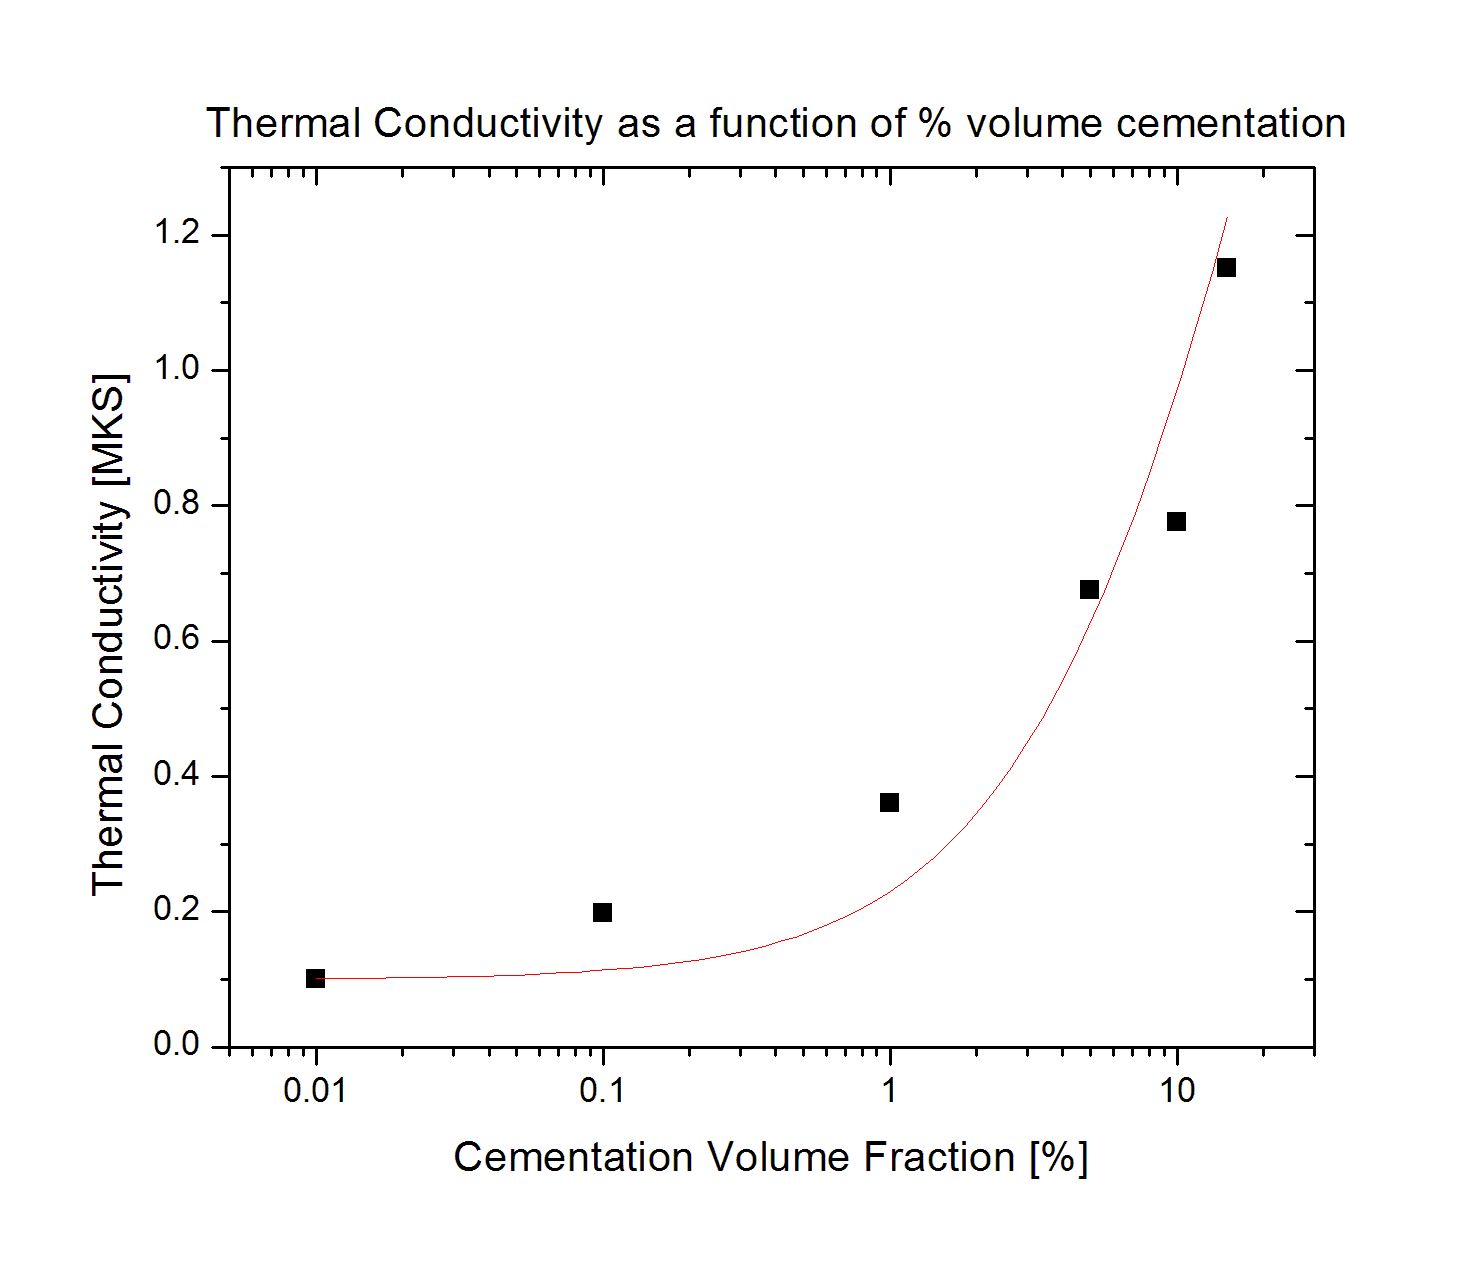
\includegraphics[width=0.57\textwidth]{PandQ2009b_CemVolumeFraction.png} }}
		\subfloat{{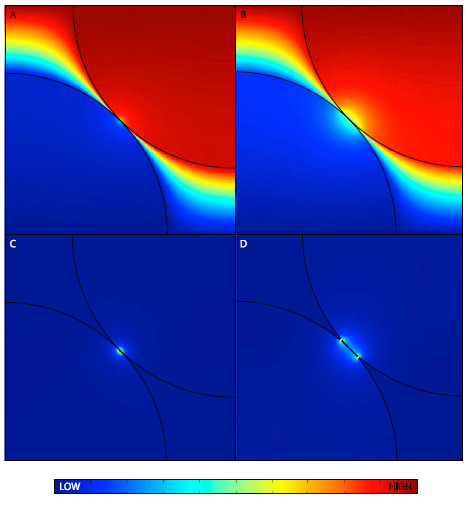
\includegraphics[width=0.43\textwidth]{PandQ2009b_Temp_grainimage.png} }}
		\caption{Thermal conductivity as a function of \% volume cementation for a 33\% porous regolith (excluding volume occupied by cementation material). The thermal conductivity of the cementation and grain material was taken to be 6 MKS and 0.937 MKS, typical of crystalline ice and silica/basaltic glass respectively. Data taken from Piqueux and Christensen (2009)}
	\end{figure}

	The plot on the left shows that the thermal conductivity of the anomalous region on Mimas ($k_{in} = 0.0113$ MKS) falls well below the minimum cement volume fraction used, not including zero cementation. However, it can be seen that, for vanishing gas conductivity,  the relationship between the cement volume fraction and thermal conductivity can be approximated by $V_{cem} \varpropto 21\cdot (k_{eff})^{3.32}$ which yields a the volume fraction, $\chi$, of cement inside the anomaly as $<1\times10^{-6} \%$.
	
	It should be noted that the grain thermal conductivity used was 0.937 MKS while the cement thermal conductivity was 6 MKS, and the packing structures investigated were all cubic regular packings. It was shown that for very low cement volume fractions the cement thermal conductivity is negligible and the effective thermal conductivity, for the ranges of \% volume cementation evaluated, approaches a single value dependent on grain size and pore gas pressure. Though the effect of varying the grain thermal conductivity was not discussed in the paper, it can be assumed to be negligible given that heat transfer between grains is limited by the point of contact. Since small cementation volume fractions of the order estimated by extrapolation were not considered, we cannot use this model for small cementation volumes due to electron heating of grains that are expected due to the low thermal conductivies of Mimas and Tethys.

\subsubsection{Maxwellian effective conductivity}
	 Wood (2011, 2013) developed a heat transfer model for grainy porous regolith based on the Maxwell equation for effective conductivity of an isotropic, heterogeneuos media. Although originally developed for electrical conductivity, the equation applies equally to thermal conductivity where the thermal paths - solid state conduction, convection through gas filled pores, and radiation from grain surfaces across pores - can be taken as acting in parallel as in \ref{eq:TCbasic}. The conductive term takes into account both solid and gas phase heat transfer and is limited depending on which phase forms a continuous path throughout the material, the lower limit corresponding to a continuous gas phase and the upper limit to a continuous solid phase. Since the lower limit is strictly valid only when the solid particles are not in contact, a non-physical situation for a regolith material, the degree of solid phase continuity is taken into account by introducing a multiplicative factor. Taking the radiative term to be negligible as discussed above, the effective thermal conductivity is given as
	
	\begin{equation}
	k_{eff} = k_{cond,min} +f_{sc}(k_{cond,max}-k_{cond,min}).
	\end{equation}
	
	For the low pressure environments of Mimas and Tethys the lower thermal conductivity limit can be taken to be zero. The upper limit depends on the thermal conductivity of the grain material $ k_{g}$, the porosity $\phi$, the volume percent and thermal conductivity of cementation region, $\chi$ and $k_{cem}$ respectively, and the fractional continuity of the solid phase $f_{sc}$. Assuming that the cementation and bulk grains are both crystalline ice ($k_{g} = k_{cem} = k_{ice}$) and that the volume percent cementation is much less than the grains ($\chi << 1-\phi$), the effective thermal conductivity becomes:	
	
	\begin{equation}
	k_{eff}=2 f_{sc} k_{ice} \frac{1-\phi}{2+\phi}
	\end{equation}
	
	The $f_{sc}$ factor represents the effect of interparticle contact and/or cementation and is a measure of the efficiency of contact between adjacent grains. The factor contains both geometrical and contact area considerations and, for uncemented soils, is given in terms of the size and number of contacts per particle, where contact size is determined by Hertzian analysis and cohesive surface forces (JKR theory).
	
	\begin{equation}
	f_{sc} = Y_{sc}N_{c} \left( \frac{N_{c}}{2\sqrt{N_{c}-1}} \frac{R_{con}}{r_{g}} \right)^{Z_{sc}}
	\end{equation}
	
	where R$_{con}$ is the radius of the contact area, r$_{g}$ is the grain radius, N$_{c}$ is the coordination number, Y$_{sc}$ is a factor determined by fitting to experimental data, and Z$_{sc}$ determines how the heat flux varies with contact radius between particles. Batchelor and O'Brien (1977) showed that the length scale for significant surface and bulk temperature variations is 
	
	$\lambda_{\nabla T} \approx \frac{r_{g}}{\alpha_{k}}$ 
	
	where 
	
	$\alpha_{k}=\frac{k_{cond}}{k_{conv}+k_{rad}}$
	
	When $R_{con} >> \lambda_{\nabla T}$, most of the heat flux is concentrated on the perimeter of the contact area and the effective thermal conductivity depends only linearly on the contact radius ($\Rightarrow Z_{sc} = 1$) [Piqueux and Christensen, 2009]. However, when $R_{con}<\lambda_{\nabla T}$ the heat flux density is constant across the contact area and the total heat flux increases as the square of the contact radius ($\Rightarrow Z_{sc} = 2$). For the case considered here, the gas and radiative thermal conductivities are quite small meaning that $\alpha_{k}$ is large and $Z_{sc} = 1$. This differs from other thermal conductivity models considered below where the thermal conductivity is assumed to depend on the square of the contact radius. 
	
	 The coordination number can be calculated exactly for regular packings of monodisperse spheres, with N$_{c}$ = 6 for simple cubic packing which has a porosity of 47.64\%, similar to the porosity used here. For polydisperse mixtures of randomly packed particles the coordination number cannot be known exactly, but for small, cohesive, nearly spherical particles Yang et al (2000) gave a functional relationship between coordination number and porosity which closely matches measured and modeled random packings, especially at porosities $\ge$40\%. 
	
	\begin{equation}
	N_{c} = 2.02 \left( \frac{1+87.38(1-\phi)^{4}}{1+25.81(1-\phi)^{4}} \right)
	\end{equation}
	
	Using a porosity of 50\%, we find the coordination number is N$_{c}$ = 4.99. We note that for non-spherical particles the shape, orientation, and roughness of a particle can have an effect on the number of contacts and thus the porosity is less strongly coupled to the coordination number. The equilibrium contact radius between two elastic spheres of the same radius R$_{s}$ under a mechanical load can be calculated from JKR theory (Johnson et al., 1991) and is discussed in more detail for non-spherical particles by Wood (2013). An averaged best fit value of Y$_{sc}$ = 0.09 with a mean standard deviation of 13.6\% was found by fitting thermal conductivity data a variety of glass bead samples of various size distributions. Using these values and assuming a mean particle size of 50$\mu$m, we can determine the solid continuity factor and the contact radius. These values are given in table 2. 
	
	Taking the ratio of the contact radius values obtained from the Wood analysis, we find $\frac{R_{cont,in}}{R_{cont,out}} = 16.9$ for Mimas, while for Tethys we find $\frac{R_{cont,in}}{R_{cont,out}} = 25.0$. Interestingly, if we take the square root of these values, we find they match closely with the values obtained below.
	
\subsubsection{Analytical solutions of the heat transfer equation}

	Solutions of the heat transfer equation for spherical geometry are complicated by radiation-conduction coupling and complex packing geometries. Chan and Tien (1973) solved the equations analytically and derived explicit functional relationships between the thermal conductance of regularly packed spheres under vacuum and fundamental system parameters. This approach was adopted by Gundlach and Blum (2012) to describe thermal conductivity of granular regoliths and compared the theoretical results with experimental data. The effective thermal conductivity was given as a function of the thermal conductivity of the solid grains, the contact radius between particles, and the packing arrangement of particles in the bulk.
	
	\begin{equation}
	k_{eff}(r_{g}, T, \phi) = k_{ice}\cdot R_{con} \cdot \xi(r_{g}, \phi)= k_{ice}(T) H(r_{g},T, \phi)
	\end{equation}

	where H is the 'Hertz-factor' used to take into account the reduction of the thermal conductivity in porous materials and the packing structure of the material and the number of interparticle contacts is taken into account by

	\begin{equation}
	\xi(r_{g}, \phi) = \frac{1}{0.531 S(\phi)} \frac{N_{A}(r_{g})}{N_{L}(r_{g})}
	\end{equation}

	Here, $S(\phi)$ is a 'model parameter' that depends on the packing structure, and $N_{A}(r_{g})$ and $N_{L}(r_{g})$ are the number of particles per unit area and unit length respectively. Applying JKR theory we can define the Hertz-factor as the ratio of the effective and bulk thermal conductivities which is slightly different than the Hertz factor described in the next section. The constants used in the packing structure dependence were only given for regular packing arrangements, and thus could not be used to the random packing considered here. Thus, the analysis of Gundlach and Blum is excluded from further analysis. 
	
\subsection{Equivalent conductance modeling}

	Another method of determining the effective thermal conductivity of a porous regolith is to consider a unit cell representative of the entire particle bed and and postulating parallel heat flux through the entire cell [Zehner, 1972; Bauer, 1976; Bauer and Schl\"{u}nder, 1978; Tsostas and Martin, 1987]. Although this is a simplification of realistic beds, it allows for inclusion of detailed parameters representing radiation and gas thermal conductivity, particle flattening, shape, and size distribution without sacrificing ease of calculation. Taking equations presented in Tsostas and Martin (1987) and, assuming low pressure (high Knudsen numbers), the effective thermal conductivity can be written

	\begin{equation}
	k_{eff} = \left(1-\sqrt{1-\phi} \right)\phi \cdot k_{void} + \sqrt{1-\phi}\left[ H k_{ice}+(1 - H)\frac{B+1}{B}\frac{k_{ice}k_{void}}{k_{ice}+k_{void}} \right]
	\end{equation}
	
	where$k_{void}$ is the thermal conductivity across the void region due to a combination of radiative heat transfer and the latent heat of sublimation, $k_{ice}$ is the thermal conductivity of bulk ice, and $H$ is the 'Hertz-factor' used to describe particle flattening at the point of contact. The deformation factor $B$ controls the shape of the solid particle portion of the unit cell and can be related to porosity by:
	
	\begin{equation}
	B = 1.25 ( \frac{1-\phi}{\phi} )^{10/9}
	\end{equation}
	
%	Note that for a porosity of $\phi = 0.5$, the deformation factor $B = 1.25$. Using the greater value of $k_{void} = 6.3\times10^{-6} \frac{J}{m \cdot s \cdot K}$ from the analysis above and a thermal conductivity for ice at 80 K of $k_{ice} = 567/T = 7.09 \frac{J}{m \cdot s \cdot K}$, we can analyze the effective thermal conductivity to obtain a comparison of the Hertz factor inside and outside the thermal anomally feature.

	Taking the thermal conductivity of the void region to be negligible as discussed above, we can simplify the effective thermal conductivity to depend only on the Hertz factor and the porosity of the regolith.
	
	\begin{equation}\label{eq:unitcell}
	\Rightarrow k_{eff} \approx \sqrt{1-\phi}\cdot H \cdot k_{ice}(T)
	\end{equation}
	
	 Using the effective thermal conductivities obtained above for a 50\% porous regolith both inside and outside the anomalies and taking the thermal conductivity of water ice at 80Kto be $k_{ice} = 567/T = 7.09$ MKS [Kossacki et al., (1994)], we can solve for the Hertz-factor (Table 1). In this instance, the Hertz-factor was taken as an empirical parameter that was determined by fitting to experimental data, and values obtained previously to describe sand particles [Tsostas and Martin, 1987] and a porous icy cometary nucleus [Steiner and K\"{o}mle, 1991] are on the order of  $H  \approx (1 - 4) \times10^{-3}$ [SteinerKomle1991] compare favorably with the values obtained for the icy regoliths considered here. Kossacki et al. (1994), using the same analysis, assumed that the Hertz-factor was related to the square of the particle contact radius so that
	
	\begin{equation}
	\Rightarrow \frac{R_{con,in}}{R_{con,out}} = (\frac{H_{n, in}}{H_{n, out}})^{1/2}
	\end{equation}
	
	from which we find that $\frac{R_{con,in}}{R_{con,out}} = 4.17$ Mimas and $5$ for Tethys, meaning the effective radius of contact is greater inside the anomalies than outside and of the same order for the two bodies.
	
\subsection{Effective Medium Theory approach}

	Thermal conductivity in porous granular regoliths has several similarities to percolation of electricity through mixed media of differing conductivities, and similar mathematical approaches can be used to study both. Below a certain volume percentage of conductive material the effective conductivity of the mixture is effectively zero, while once a certain critical concentration is reached the conductivity increases sharply and continues to increase with increasing volume percent of conductive material. The material can be viewed as an effective-medium to estimate the effective thermal conductivity for a random network of spherical grains arranged on a regular lattice  [Sirono and Yamamoto, 1997; Kirkpatrick, 1973]. Integrating the probability distribution of $k$ multiplied by the 1-D heat flux to obtain the effective heat flux and taking the thermal conductivity of the void space to be zero, the effective thermal conductivity is given by
	
%	\begin{equation}
%	\frac{k_{eff} - k_{ice}}{k_{ice} +(1/p_{c}-1)k_{eff}}p + \frac{k_{eff}-k_{void}}{k_{void}+(1/p_{c}-1)k_{eff}}(1-p)=0
%	\end{equation}
	\begin{equation}
	k_{eff} = k_{ice} \frac{p - p_{c}}{1 - p_{c}}
	\end{equation}

	where the probability of a lattice site being occupied or packing fraction is $p$ and $p_{c}$ is the percolation threshold which defines the minimum packing fraction for a continuous thermal path to exist across the material. However, this expression does not consider the limitation of heat flow due to reduced area at the grain contacts. This effect can be taken into account by multiplying by a factor dependent on packing structure, grain size and effective contact radius similar to that found by Hertzian analysis.
	 
	\begin{equation}
	k_{eff} = k_{ice} ( \frac{p - p_{c}}{1-p_{c}} )\frac{\pi R_{con}^{2}}{g r_{g}^{2}}
	\end{equation}

	where $g$ is a geometrical factor dependent on the packing structure and $g = 4$ for a cubic lattice. Assuming a simple cubic packing structure of the grains, the relation between porosity and the packing fraction is
	
	\begin{equation}
	p = \left[ \frac{4 \pi}{3} \left( \frac{1}{2} \right)^{3} \right]^{-1} (1 - \phi) \\
	\end{equation}
	
	and the critical packing fraction $p_{c} = 1/3$. The contact radii calculated using this method are given in table 1, and the ratio of the contact radius inside and outside the anomaly is $\frac{R_{con,in}}{R_{con,out}} = ( \frac{S_{in}}{S_{out}} )^{1/2} = 4.14$ for Mimas and $5.0$ for Tethys. This is in very close argreement with the value obtained from the analysis of Kossacki et al.

	\begin{table}
		\hspace{-1.5 cm}{
		\begin{tabular}[ h, font=small ]{ l | l | c | c | c | c | c }
	\multicolumn{2}{c | }{Authors} & Howett (2011, 2012) & \multicolumn{2}{ | c |}{Wood (2013)} & S\&K (1991) & S\&Y (1997) \\ \hline
	& Location & $k_{eff} \left[ \frac{J}{m\cdot s\cdot K} \right]$ & $f_{sc}$ & $R_{con} [\mu m]$ & H [cm$^{-1/3}$] & S [$\mu m^{2}$]\\  \hline
	Mimas & Inside anomaly & $1.13 \times 10^{-2}$ & $3.98 \times 10^{-3}$ & 0.354 & $2.25 \times10^{-3}$ & 17.1 \\
		& Outside anomaly & $< 6.7 \times 10^{-4}$ &  $2.36 \times 10^{-4}$ & .021 & $1.3 \times10^{-4}$ & 1.00 \\ \hline
	Tethys & Inside anomaly & $1.63 \times 10^{-3}$ &  $5.75 \times 10^{-4}$ & 0.051 & 3.25 $\times10^{-4}$ & 2.47 \\
		& Anomaly boundary &  $3.16 \times 10^{-4}$ &  $1.11 \times 10^{-4}$ & 0.028 & 6.30 $\times10^{-5}$ & 0.48 \\
		& Outside anomaly & $6.53 \times 10^{-5}$ &  $2.30 \times 10^{-5}$ & 0.006 & 1.30 $\times10^{-5}$ & 0.01 \\
	\end{tabular} }
	\caption{Contact radii calculated using the various thermal conductivity theories presented above. For all analyses, we see that the contact area inside the anomalous region is greater than without, which is in agreement with the increased thermal conductivity for all other factors being constant.}
	\end{table}

\section{Energy deposition due to $>$1 MeV electrons and Ice Grain Sintering}
	Steiner and K\"{o}mle (1993) gave the energy balance at the surface of an uncovered, porous water ice regolith as
	
	\begin{equation}
	\Phi = \left( - k_{eff} \frac{\partial T}{\partial z} \right) + Z^{w}L^{w} +\epsilon \sigma T_{surf}^{4}
	\end{equation}
	
	where $\Phi$ is the energy flux incident on the surface of the regolith, $Z^{w}$ is the free sublimation rate of water ice given by the Hertz-Knudsen formula, $L^{w}$ is the latent heat of water ice, and $\epsilon$ is the IR emissivity. The Hertz-Knudsen formula gives the rate of phase change (i.e. rate of molecular desorption) for a given interface which, for a low pressure solid/vapor boundary such as that considered here, was estimated by Tschudin (1946) as
	
	\begin{equation}
	Z^{w} = P_{s}(T)\frac{M}{\sqrt{2\pi R T}}
	\end{equation}
	
	where $P_{s}(T)$ is the saturation vapor pressure and M is the molecular weight.
	
	\emph{What is the expected heating rate/area per electron interaction with the ice? How close does the interaction have to be to the surface to desorb a water molecule? Can we obtain an average desorption rate due to electronic interactions?}

	Paranicas et al (2012) estimated the energy flux of electrons deposited on the leading hemispheres of Mimas and Tethys to be $1.21\times 10^{12} \frac{eV}{cm^{2}\cdot s}$ and $1.91\times 10^{11} \frac{eV}{cm^{2}\cdot s}$ respectively. However, not all of the energy is deposited in the surface region as the electrons penetrate up to cm depths into the sample. Therefore, the energy loss occurs as a function of depth in the materials and is transfered to the ice grains as ionizations or excitations of the constituent atoms which in turn can create defects in the crystal structure and heat the grains. The interactions of electrons with the water molecules can change as a function of energy. The deposition of energy into the ice grains can lead to sintering of the grains by enhanced diffusion of atoms through the bulk or along the surface of the grain and desorption of atoms or molecules at the surface which are subsequently redeposited with some probability in the neck region. A total of six such mechanisms (Fig.~\ref{fig:diffmech}) were identified by Swinkels and Ashby (1981) which can be further classified into densifying and non-densifying mechanisms.
	
	\begin{figure}
	\centering
		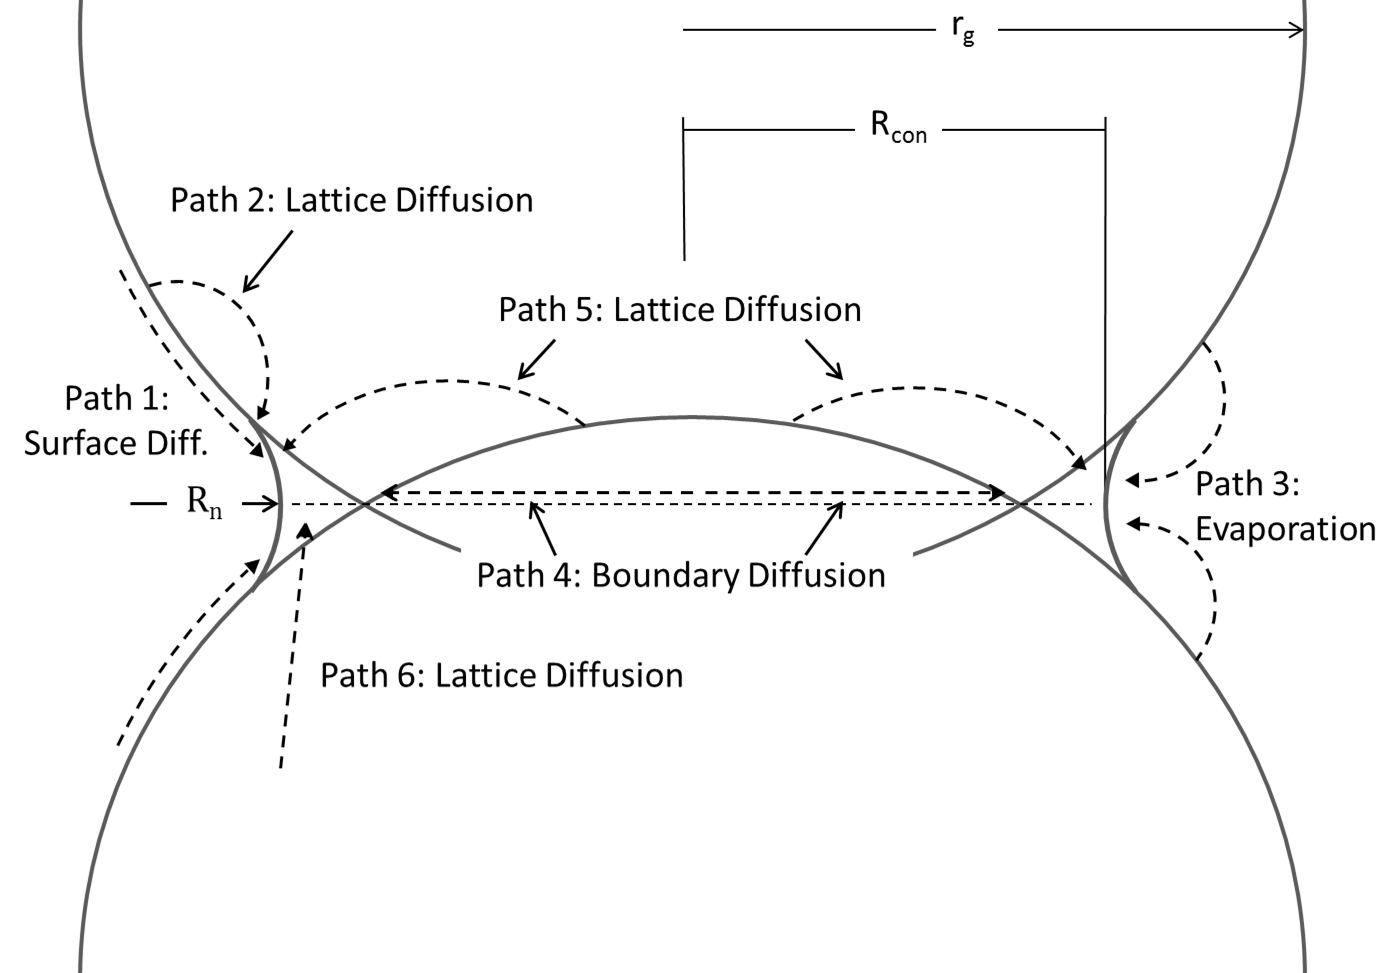
\includegraphics[scale=0.5]{Swinkels1981_DiffMech.png}
	\caption{Pictoral description of the six sintering mechanisms defined by Swinkels and Ashby (1981) who estimated that the defining equations for the various mechanisms (defined below) were acurate to within a factor of 2.}
	\label{fig:diffmech}
	\end{figure}
	
	\begin{itemize}
	\item Non-densifying Mechanism
		\begin{enumerate}
		\item Surface diffusion from a surface source \\
	$\dot{V_{1}} = \frac{3 \pi R_{con} \delta_{s} D_{s}\gamma_{s} \Omega (K_{3}-K_{2})}{d_{2}k_{B}T}$
		\item Lattice diffusion from a surface source \\
	$\dot{V_{2}} = \frac{3 \pi R_{con} D_{v}\gamma_{s} \Omega (K_{3}-K_{m})}{k_{B}T}$
		\item Vapour transport from a surface source \\
	$\dot{V_{3}} = 2 \pi R_{con} R_{n} \theta P_{v} \frac{\gamma_{s} \Omega}{k_{B}T}\left[ \frac{\Omega}{2 \pi \rho_{b} k_{B}T} \right]^{1/2} (K_{3}-K_{m})$
		\end{enumerate}
	\item Densifying Mechanism
		\begin{enumerate}
		\setcounter{enumi}{3}
		\item Grain boundary diffusion from a bourdary source \\
	$\dot{V_{4}} = \frac{16\pi \delta_{b} D_{b}\gamma_{s}\Omega}{R_{con}k_{b}T}\left(1-\frac{K_{1}R_{con}}{2}\right)$
		\item Lattice diffusion from a boundary source \\
	$\dot{V_{5}} = \frac{32\pi R_{n} \theta D_{v}\gamma_{s}\Omega}{R_{con}k_{b}T}\left(1-\frac{K_{m}R_{con}}{2}\right)$
		\item Lattice diffusion from dislocation sources \\
	$\dot{V_{6}} = \frac{8\pi R_{con}^{2} R_{n} \theta N D_{v}\gamma_{s}\Omega}{9 k_{b}T}\left(-K_{m}-\frac{3 \tau R_{con}}{2 \gamma_{s} r_{g}}\right)$
		\end{enumerate}
	\end{itemize}
	
	where
	
	\begin{itemize}
	\item	$R_{n}$ = neck curvature radius ($cm$) 
	\item	$K_{1-3}$ = "curvatures" defined for specific geometry ($cm^{-1}$) 
	\item	$K_{m}^{2}$ = $K_{1}K_{2}$ 
	\item	$\delta_{s}$ = effective surface thickness ($cm$) 
	\item	$\delta_{b}$ = effective grain boundary thicknesss ($cm$) 
	\item	$D_{s}$ = surface diffusion coefficient ($cm^{2}/s$) 
	\item	$D_{v}$ = lattice diffusion coefficient ($cm^{2}/s$) 
	\item	$D_{b}$ = grain boundary diffusion coefficient ($cm^{2}/s$) 
	\item	$\gamma_{s}$ = surface free energy ($J/m^{2}$) 
	\item	$\gamma_{b}$ = grain boundary free energy ($J/cm^{2}$) 
	\item	$\rho_{b}$ = bulk density ($g/cm^{3}$) 
	\item	$\Omega$ = molar volume ($cm^{3}$) 
	\item	$\mu$ = molar mass ($g$)  
	\item	$\tau$ = shear modulus ($dyne/cm^{2}$) 
	\item	$N$ = dislocation density ($cm^{-3}$) 
	\end{itemize}
	
	The rate of growth of the neck region between grains is thus a function of the energy deposition rate and by extension by the various diffusion and desorption rates of atoms and molecules into the contact region.
	
	\begin{equation}
	\frac{dR_{con}}{dt} = \dot{R_{con}} = \frac{\sum_{i=1}^{6} \dot{V_{i}}}{2\pi R_{con} \theta \rho}
	\end{equation}
	
	Kossacki et al (1994) gave an estimate for the neck growth rate due to vapor transport driven by thermal desorption from the grain surface. Vapor desorption and redeposition is likely the dominant sintering mechanism at $\sim$200K, though it may not be relevant at Mimas surface temperatures.
	
	\begin{equation}
	\dot{V_{3}} = \frac{\Omega^{2}\gamma p A_{n}}{(2\pi\mu RT)^{1/2}RT} \left( \frac{2}{r_{g}} + \frac{1}{\rho_{b}} - \frac{1}{R_{con}} \right)
	\end{equation}
	
	The pressure $p$ due to sublimation of molecules from the pore surfaces can be calculated using the Clausius-Clapeyron equation given earlier (Eq.\ref{eqn:CCpres}), and the the neck surface area is given by
	
	\begin{equation}
	A_{n} = 4\pi\rho \left[ (R_{con} + \rho)arcsin\left(\frac{r_{a}}{\rho}\right) - r_{a} \right]
	\end{equation}
	
	where $r_{a}$ and $\rho$ are defined by
	
	\begin{equation}
	\rho = \frac{R_{con}^{2}}{2(r_{g}-R_{con})}
	\end{equation}
	
	and
	
	\begin{equation}
	 r_{a} = \frac{r_{g}\rho}{r_{g}+\rho}
	\end{equation}
	
	\emph{I think the goal here should be to relate the warming of the grain due to a electron ineratction with the regolith to a average desorption rate. I am imagining this as the number of electeron interactions per surface area per time, multiplied by an average number of desorbed molecules per event to give number of desorbed molecules per area per time.}
	
	The electronic structure of ice at the interface of large porous cavities in amorphous ice may resemble that of the free surface interface, and therefore it might be expected that ESD processes would occur there with similar mechanisms. The total ESD neutral product yields are generally much higher from amorphous ice than from crystalline. This is attributed to increased defect density and an increase in excitation localization due to disruption of long range order in the matrix [Sieger and Orlando, Surf. Sci. 451(2000) 97].

\section{Regolith gardening rate}


\newpage

\section{Appendiux 1: Review of measured Parameters}
\label{sec:measured}

\subsection{Thermal Inertia (I) - Howett et al. (2011)}
\label{sec:inertia}

	\begin{equation}
	I = \sqrt{kc\rho} \: [\frac{J}{m^{2} K^{1} s^{1/2}}]
	\end{equation}

	\hspace{1cm}
	Where
	\begin{itemize}[leftmargin=3cm]
	\item k = thermal conductivity $[\frac{J}{m \cdot s \cdot K}]$
	\item c = specific heat $[\frac{J}{g \cdot K}]$
	\item $\rho$ = density $[\frac{g}{m^{3}}]$
	\end{itemize}

	The thermal inertial measured by Cassini CIRS was reported by Howett et al. (2011, 2012)
	\begin{itemize}
		\item For Mimas:
		\begin{itemize}
			\item Within anomaly: \fbox{$66 \pm 23  [\frac{J}{m^{2} K^{1} s^{1/2}}]$}
			\item Outside anomaly: \fbox{$< 16  [\frac{J}{m^{2} K^{1} s^{1/2}}]$}
		\end{itemize}
		\item For Tethys:
		\begin{itemize}
			\item Within anomaly: \fbox{$25 \pm 3$ MKS}
			\item Anomaly boundary: \fbox{$11 \pm 1$ MKS}
			\item Outside anomaly: \fbox{$5 \pm 1$ MKS}
		\end{itemize}
	\end{itemize}
		
	\emph{Depth of penetration for CIRS wavelength light?}
	
\subsection{Temperature ranges - Howett et al. (2011)}
\label{sec:temperature}

	Estimated Mimas daytime temperatures: 40-95 K
	
\subsection{Average Particle Size}
\label{sec:size}

%In the UV, Mimas is nearly as bright as Enceladus. Tethys is surprisingly dark in the UV.
%Modeling (Hamilton and Burns, 1994) showed that e-ring grains at the orbit of Mimas (inside the 3.95 R$_{s}$ orbit of Enceladus) are expected to coat the trailing hemisphere of the moon, while at Tethys and other satellites exterior to Enceladus, the e-ring grains impact primarily on the leading hemispheres. 
	
Particle size (diameter) measured using the Cassini observations and, assuming pure water ice regoliths, comparing the water ice absorption band depths at 2.0$\mu m$ and 1.52$\mu m$ to a model correlating absorption depth to grain size developed by Clark and Lucey (1984).

	\begin{itemize}
	\item Mimas: (Hendrix et al, 2012)
	\begin{itemize}
		\item Leading hemisphere: 20-80 $\mu$m
		\item Trailing hemisphere: 10-50 $\mu$m
		\item Herschel crater: 50-100 $\mu$m
	\end{itemize}

	\item Tethys: (Fillachione et al, 2012)
	\begin{itemize}
		\item Average: 30 $\mu$m
		\item Pure H$_{2}$O ice: 22 - 880 $\mu$m
		\item Mixed grains: 69 $\mu$m
	\end{itemize}

	\item Dione (assuming pure water ice): (Newman et al, 2009)
	\begin{itemize}
		\item Whispy region: 6-28 $\mu$m
		\item Dark area: 1-8 $\mu$m
		\item Background: 7-28 $\mu$m
	\end{itemize}
	\end{itemize}

\subsection{Porosity}
\label{sec:porosity}

	The density of a porous medium is given by $\rho_{\phi} = \rho_{0}*(1-\phi)$ where $\rho_{0}$ is the density of the bulk substance. 

	\begin{itemize}
	\item For Enceladus - Verbischer et al (2005): $~50-70\%$
	\item For Tethy's - Caravano et al. (2007): $>90\%$ 
	\item Model parameter (ansatz) Leliwa-Kopystynski (2000): $~50\%$
	\end{itemize}
	
\subsection{Density}

\section{List of Variables}
$\phi$ = porosity
$\chi$ = cementation volume fraction
$\nu_{s}$ = solid volume fraction

\section{Tabulated Literature Parameters}
\label{sec:tabulated}
	
\subsection{Thermal Conductivity}
\label{sec:tconductivity}
	
	Low temperature thermal conductivity
	
	\begin{itemize}
	\item Water Ice
		\begin{itemize}
		\item Ellsworty and Schubert (1983): $k_{ice} = \frac{488.12}{T} +0.4685 \: [\frac{J}{m s K}]$
		\item Haruyama et al (1993) via. Sirono and Yamamoto (1997):
			\begin{itemize}
			\item Amorphous: $k_{H_{2}O, a} = k_{ao} \times T$ where $k_{ao} = 7.1x10^{-3} \: [\frac{erg}{cm s K}]$
			\item Crystalline: $k_{H_{2}O, c} = k_{co}/T$ where $k_{co} = 5.67x10^{7} \: [\frac{erg}{cm s K}]$
			\end{itemize}
		\item Kossacki et al. (1994): $k = \frac{567}{T} \: [\frac{J}{m s K}]$
		\item Klinger (1975): $k_{100 K} = 0.04  \: \frac{J}{m s K}$ (amorphous)
		\end{itemize}
%	\item Silicates
%		\begin{itemize}
%		\item Basalt
%			\begin{itemize}
%			\item Clauser (1995) - Bulk: k $\approx 1.5 - 3.5 [ \frac{J}{m \cdot s \cdot K}]$
%			\item Fountain and West (1970) - Crushed (37-62 $\mu m, \rho = 0.9 g/cm^{3}$, T=150K): k $\approx 7\times10^{-4} [\frac{J}{m \cdot s \cdot K}]$
%			\end{itemize}
%		\item Quartz
%			\begin{itemize}
%			\item engineeringtoolbox.com - Bulk: k $\approx 3.0 [\frac{J}{m \cdot s \cdot K}]$
%			\item Smoluchowski (1910) - Crushed (94$\mu$m): k $\approx 3.0 [\frac{J}{m \cdot s \cdot K}]$
%			\end{itemize}
%		\item Pumice
%			\begin{itemize}
%			\item  Hemmings et al. (2009) - Bulk: k $\approx 0.4269 [\frac{J}{m \cdot s \cdot K}]$
%			\item Wechsler and Glaser (1965) - Crushed (44-104 $\mu$m): 
%			\end{itemize}
%		\end{itemize}
	\end{itemize}

\subsection{Specific  and Latent Heat}
\label{sec:sheat}

	Low temperature specific heat:
	
	\begin{itemize}
	\item Ramirez et al. (2012): $c_{100 K} ~ 0.83 [\frac{J}{g K}]$
	\item NBS Monograph 21 (): $c_{100 K} = 0.82 [\frac{J}{g K}]$
	\item Gutierrez et al. (2001): $c_{H_{2}O} = (0.9 + 0.00749 * T) [\frac{J}{g K}]$
		$\rightarrow c_{H_{2}O}(80K) = 1.50 J/g\cdot K$
	\end{itemize}
	
	Latent heat of sublimation:
	
	\begin{itemize}
	\item Gutierrez et al. (2001): $L = 48600 [\frac{J}{mol}]$
	\end{itemize}

\section{Appendix 2: Calculations}

\begin{itemize} 
\item Skin Depth (calculated for Mimas - outside anomaly)
\begin{equation}
\begin{split}
\delta_{out} &= \frac{I_{out}}{\rho_{regolith} c \sqrt{\omega}}  \\
&= \frac{I_{out}}{(1-\phi)\rho_ {ice} c \sqrt{\omega}} \\
&= \frac{16[\frac{J}{m^{2} s^{1/2} K}]}{(1-0.5)0.934[\frac{g}{cm^{3}}]0.8[\frac{J}{g \cdot K}]\sqrt{7.7\time10^{-5}[\frac{rad}{s}]}} \\
\Rightarrow \delta_{out}&= 0.49\: [cm]
\end{split}
\end{equation}

\item Radiative thermal conductivity
	\begin{equation}
	\begin{split}
	\Rightarrow \epsilon' &= 1 \\
	\Rightarrow \psi &= \frac{1+F}{1-F} \approx 1.087 \\
	\Rightarrow k_{rad} &= 4 (1.087)(5\times10^{-5} m)(5.67\times10^{-8} \frac{J}{m^{2} s K^{4}}(80 K)^{3}) \\
	\Rightarrow k_{rad} &= 6.3\times10^{-6} \frac{J}{m \cdot s \cdot K}
	\end{split}
	\end{equation}

\item Sublimation Heat Transfer
	\begin{equation}
	\begin{split}
	k_{lat} = [ \frac{18 \frac{g}{mol} \times N_{A}}{2 \pi k_{b} (80K)} ]^{1/2} (48600 \frac{J}{mol} & \times N_{A})(0.9 \cdot 50\times10^{-6} m) [ \frac{(3.56\times 10^{12} \frac{N}{m^{2}})(6141.7 K)}{(80 K)^{2}} exp( \frac{-6141.7}{80} ) ] \\
	\Rightarrow k_{lat} &= 1.15\times10^{-26}\frac{J}{m \cdot s \cdot K}
	\end{split}
	\end{equation}

\item Wood 2011 simplification
	\begin{equation}
	\begin{gathered}
	k_{c,max} = k_{ice} \frac{\chi + 1 - \phi}{\chi + 1 + \frac{\phi}{2}} \\
	\Rightarrow k_{eff} = f_{sc} k_{c,max} = f_{sc} k_{ice} \frac{\chi + 1 - \phi}{\chi + 1 + \frac{\phi}{2}} \\
	\\
	\text{assuming   } \chi << \phi  \Rightarrow k_{eff}=2 f_{sc} k_{ice} \frac{1-\phi}{2+\phi}
	\end{gathered}
	\end{equation}

\item Steiner and K\:{o}mle 1991 simplification
	\begin{equation}
	\begin{gathered}
	k_{eff} = (1-\sqrt{1-0.5})(0.5)(6.3\times10^{-6}) + \sqrt{1-0.5} [ H \cdot 7.09+(1-0.5)\frac{1.25+1}{1.25}\frac{(7.09)(6.3\times10^{-6})}{(7.09+6.3\times10^{-6})} ] \\
	\Rightarrow k_{eff} = ( 4.93\times 10^{-6} + 2.24\cdot H )  \frac{J}{m \cdot s \cdot K} \\
	\Rightarrow k_{eff} \approx \sqrt{1-\phi}\cdot H \cdot k_{ice}(T)
	\end{gathered}
	\end{equation}

\item Sirono and Yamamoto 1997 expression variations
	\begin{equation}
	\begin{gathered}
	k_{eff}=k_{ice}\left( \frac{p-p_{c}}{1-p_{c}} \right) \frac{\pi R_{con}^{2}}{gr^{2}} \\
		 =k_{ice}\left( \frac{p-p_{c}}{1-p_{c}} \right) \frac{\pi}{g r^{2}} H^{2} \\
		 = k_{ice}\left( \frac{p-p_{c}}{1-p_{c}} \right) \frac{\pi}{g r^{2}}[ \frac{9 \pi \gamma r^{2} (1-\mu^{2})}{8 E} ]^{2/3}
	\end{gathered}
	\end{equation}
	
\item Sirono and Yamamoto Contact Area
	\begin{equation}
	\begin{gathered}
	S_{in} = \frac{k_{eff, in}}{k_{ice}} \frac{1-p_{c}}{p - p_{c}}\cdot g r_{grain}^{2} \\
	= \frac{0.00113}{7.09} \frac{1-1/3}{0.955-1/3} \cdot (4)(50 \mu m)^2 \\
	\Rightarrow S_{in} = 1.71\times 10^{-11} m^{2} \\
	\Rightarrow S_{out} = 1.00\times 10^{-12} m^{2}
	\end{gathered}
	\end{equation}
	
\item Grain radius simplification
	\begin{equation}
	\begin{split}
	\frac{H_{in}}{H_{out}} &= \frac{k_{in}}{k_{out}} = \frac{r_{in}^{2/3} \xi(r_{in}, \phi)}{r_{out}^{2/3} \xi(r_{out}, \phi)} \\
	\Rightarrow \frac{H_{in}}{H_{out}} &= \frac{r_{in}^{2/3} \frac{N_{A}(r_{in})}{N_{L}(r_{in})}}{r_{out}^{2/3} \frac{N_{A}(r_{out})}{N_{L}(r_{out})}} \\
	& \text{where }\: N_{A}\varpropto \frac{1}{r^{2}} \: \text{and} \: N_{L}\varpropto \frac{1}{r} \\
	\Rightarrow \frac{r_{in}}{r_{out}} &= (\frac{H_{out}}{H_{in}})^{3}
	\end{split}
	\end{equation}

\item Gundlach and Blum 2012 extension of Hertz analysis to aggregates
	 This thermal conductivity equation can be modified to describe a porous regolith layer composed not simply of spherical grains, but of grain aggregates which themsleves are composed of ice grains and which have their own unique materials parameters such as volume filling factor, Poisson's ratio, Young's modulus, and specific surface energy. Taking the volume filling factor (V$_{F}=1-\phi$) of the layer to be the product of the volume filling factors of the aggregates themselves and the volume filling factor of the aggregate structure ($V_{F, layer} = V_{F, agg} V_{F, struc}$), we can write the effective thermal conductivity of the layer as:
	 
	 \begin{equation}
	 \begin{split}
	 k_{layer}(r_{0}, R, T, V_{F, struc}, V_{F, agg}) = \\
	 k_{agg}(r_{0}, T, V_{F, agg}) [\frac{9}{4} \frac{1 - \mu_{agg}^{2}}{E_{agg}(T)}  \pi \gamma_{agg}(T) r^{2}]^{1/3} \xi(R, V_{F, struc})
	 \end{split}
	 \end{equation}
	 
	 where $R$, $E_{agg}$, and $\mu_{agg}$ are the radius, Young's modulus, and Poisson's ratio of the aggregates, respectively. Taking $r_{0}$ to be the grain radius (the size of the grains that make up the aggregate), the specific surface energy of the aggregates can be calculated by:
	 
	 \begin{equation}
	 \gamma_{agg}(T) = V_{F, agg} \gamma_{ice}^{5/3}(T)[\frac{9 \pi (1-\mu_{agg}^{2})}{r_{0} E_{ice}(T)}]^(2/3)
	 \end{equation}
	 
	 The thermal conductivity of the aggregates can be calculated as before:
	 
	 \begin{equation}
	 k_{eff}(r_{0}, T, V_{F, agg} = k_{ice}(T) [\frac{9 (1-\mu_{ice}^{2})}{4 E_{ice}(T)}\pi \gamma_{ice}(T) r_{0}^{2} ]^{1/3}\xi(r_{0}, V_{F, agg})
	 \end{equation}

\end{itemize}

\section{Appendix 3: Summary of thermal conductivity models}
 Conductivity through grains is limited by the contact area between adjacent grains. Several models are discussed in the following and summarized here for ease of comparison.
	
	\begin{itemize}
	\item Wood (2013)
		\begin{equation}
		k_{eff}  = f_{sc} k_{ice} \frac{\chi + 1 - \phi}{\chi + 1 + \frac{\phi}{2}} \\
		\end{equation}
		
		where $\chi$ is the volume fraction of cement. Taking $\phi = 0.5$ and assuming $\chi << \phi$ this equation simplifies to $k_{eff} \approx \frac{2}{5} f_{sc} k_{ice}$.  The solid continuity factor $f_{sc}$ is a measure of the efficiency of heat transfer through contacts between adjacent grains and is dependent on geometrical packing and contact area, determined by Hertzian analysis and cohesive surface forces (JKR theory), between adjacent grains.
		
		\begin{equation}
		f_{sc} = Y_{sc}N_{c} \left( \frac{N_{c}}{2\sqrt{N_{c}-1}} \frac{R_{con}}{r_{g}} \right)^{Z_{sc}}
		\end{equation}
	
	Here, R$_{con}$ is the radius of the contact area, r$_{g}$ is the particle radius, N$_{c}$ is the coordination number, Z$_{sc}$ depends on the ratio of solid to void thermal conductivities and, in the case considered here of low temperature and pressure, can be taken to be 1, and the $Y_{sc}$ factor is a fit to experimental data. %The coordination number can be calculated exactly for regular packings of monodisperse spheres, with N$_{c}$ = 6 for simple cubic packing, and for small, cohesive, nearly spherical particles Yang et al (2000) gave a functional relationship between coordination number and porosity which closely matches measured and modeled random packings, especially at porosities $\ge$40\%. 
	
%	\begin{equation}
%	N_{c} = 2.02 \left( \frac{1+87.38(1-\phi)^{4}}{1+25.81(1-\phi)^{4}} \right)
%	\end{equation}
		
%	\item  Piqueuz and Christensen (2009b) \\
%		P and Q did not give explicit equations to calculate the thermal conductivity, but provided several larger plots that traced how the thermal conductivity varied with \% cementation, grain size, gas pressure etc. However, their focus was on ~atm pressure environments, and the model failed for very small grain contact areas (low thermal conductivities), and thus is was determined this model was unfit to explain the regolith at Mimas.

	\item Steiner and K\"{o}mle (1991)
		\begin{equation}
		 k_{eff} = \sqrt{1-\phi}\cdot H \cdot k_{ice}(T)
		\end{equation}
		
	Where H is the Hertz factor which determines the contact area between touching grains. Taking $\phi = 0.5$, we can simplify this equation to $ k_{eff} \approx 0.71 H k_{ice}$. The $\sqrt{1-\phi}$ factor of the Steiner and K\"omle model is the only term used to account for the structure of the material.

	\item Gundlach and Blum (2010)
	The Gundlach and Blum model was developed using a mathematical analysis by Chan and Tien (1973) for regularly packed spheres whose contact area is described by Hertzian analysis and where the cohesive forces between spheres are described by JKR theory.
	
		\begin{equation}
		k_{eff} = k_{ice} H \frac{1}{0.531 S(\phi)} \frac{N_{A}}{N_{L}}
		\end{equation}
		
	The factors S$_{\phi}$, N$_{A}$, and N$_{L}$ depend on the specific packing arrangement and can be computed explicitly for regular packing arrangements and H is the Hertz factor. 
	
		\begin{equation}
		 H = [\frac{9}{4} \frac{1-\nu^{2}}{E} \pi \gamma r^{2} ]^{1/3}
		\end{equation}
	
	
	\item Sirono and Yamamoto (1997)
		\begin{equation}
		k_{eff} = k_{ice} \left( \frac{p - p_{c}}{1-p_{c}} \right) \frac{\pi R_{con}^{2}}{g r^{2}}
		\end{equation}
		
		Where R$_{con}$ is the grain contact radius as defined by Hertzian analysis and $p$ is related to the volume filling factor and dependent on the packing. More specifically, $p$ is the probability that a lattice site is occupied with a regolith grain. The Hertz factor used by Sirono and Yamamoto is slightly different than that of Gundlach and Blum:
		
		\begin{equation}
		H = [ \frac{9 \pi \gamma r^{2} (1-\nu^{2})}{8 E} ]^{1/3}
		\end{equation}
		
	\end{itemize}
	
\end{document}